\subsection{What is Clustering}
Clustering is the process of grouping a set of objects into classes of similar 
objects that are meaningful, useful or both \citep{tan05}.

A cluster is a collection of objects that are similar (or related) to one 
another within that same cluster and are dissimilar (or unrelated) to other 
objects within other clusters. The more distinct the similarity within a group, 
and the greater difference between groups, the more distinct the final clustering 
will be \citep{han06}.

Cluster analysis can be found in many areas, even fundamentally in the 
development of humans. From a young age, we learn how to distinguish between 
different types of animals, such as cats and dogs \citep{han06}. 

We have been able to do this by continuously clustering the data objects. Every
time we discovered a new attribute of that object, we would subconsciously 
improve our clustering schemes \citep{han06}. 

Cluster analysis is actively used in various industries, such as social sciences, 
biology, statistics, machine learning, data analysis, market research and pattern 
recognition \citep{han06}.

Cluster analysis has been used within a biological environment for many years. 
It can be used to categorise genes with similar (or dissimilar) functionality, 
and gains insights into structures that are inherent within certain groups of 
populations \citep{han06}.

Clustering can also be used for outlier detection. An outlier is a value that 
is a large distance from any given cluster. These outliers can be of more 
interest than the actual clusters \citep{tan05}. 

Fraud monitoring systems will try to find exceptional credit card transactions 
(such as highly expensive or frequent purchases) by clustering the common 
(or ``accepted'') purchases together. This would then allow better 
identification of the unexpected purchases \citep{tan05}.

The defining of a cluster is the most important, and yet the hardest part of 
any application. Figure \ref{fig:clusterDefinition} shows twenty points, and 
three different ways of separating them into clusters, in which each cluster 
membership is deduced by its colour.

\begin{figure}[H]
  \begin{center}
    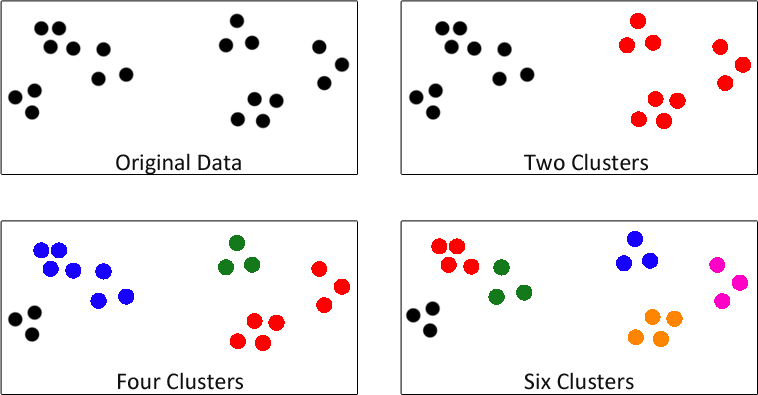
\includegraphics[width=0.80\textwidth]{chapter3/clustering/ClusterDefinition1.png}
    \label{fig:clusterDefinition}
    \caption
      {Different ways of clustering the same set of points.}
  \end{center}
\end{figure}

We can easily separate the original points into two clusters; however on closer 
inspection it appears that the two clusters have further clusters inside them. 
This figure illustrates the important fact that the definition of a cluster is 
imprecise. The definition of a cluster is not only specific to the nature of the 
data but the required results as well.